\documentclass[a4paper, 11 pt, article, accentcolor=tud7b]{tudreport}

\usepackage[utf8]{inputenc}
\usepackage{amsmath}

\title{CNuVS Exercise 11}
\author{Nils Rollshausen, Daniel Drodt}
\subtitle{Nils Rollshausen, Daniel Drodt}

\begin{document}
	\maketitle
	\section{Multicast}
	\subsection*{a) Multicast applications}
	Possible use-cases for multicast are video-conferencing applications (where video streams have to be broadcast so several participants), live-streaming (where a broadcasting station sends to many receivers) or pub/sub systems in which a server wants to notify (or push content to) many subscribers.
	  
	\subsection*{b) Multicast approaches}
	Multicast can be implemented as 'Multicast via Unicast', where the sender sends the data to every recipient separately, Network Multicast, where the routers in the network duplicate data packets and deliver them to every subscribed node, or Application Layer Multicast, where receivers can forward data to other (topographically close) receivers.
	
	\subsection*{c) Multicast routing and delivery}
	Possible approaches to multicast routing are flooding, group-shared trees or source-based trees.
	
	\subsection*{d) Steiner trees}
	While Steiner trees can be efficiently (heuristically) calculated, doing so requires knowledge of the global network state, which is usually not known to the network nodes. Additionally, the Steiner tree would have to be re-calculated on every change in network topology.
	
	\subsection*{e) ACKs}
	Acknowledgements are not used in multicast because, due to its one-to-many nature, sending ACKs for every packet would easily overwhelm the sender as the amount of ACKs scales with the number of subscribed hosts. \\
	Instead, multicast operates on the assumption that packets usually arrive and only sends negative ACKs when a node can tell that it missed a packet.
	
	\subsection*{f) IGMP}
	The protocol used to join local multicast groups is the Internet Group Management Protocol (IGMP). To join a group, the host sends an IGMP report to the router, informing it that it now wants to receive messages for a certain group. In regular intervals, the router will send a IGMP query, checking whether there are still nodes on the network interested in a particular group. Otherwise, the router will eventually stop forwarding packets for that group.
	
	\subsection*{g) Multicast IP block}
	The address range from 224.0.0.0 to 239.255.255.255 is reserved for multicast.
	
	\subsection*{h) Usable multicast addressses}
	Out of the above range, the subrange from 224.0.0.0 to 224.0.0.255 is not usable either because it is reserved or used for routing and group maintenance.
	
	\subsection*{i) ICMP error messages}
	Multicast communications never generate ICMP error messages for similar reasons as they do not generate ACKs.
	
	\section{Core Based Trees}
	
	\subsection*{a) Multicast from A}
	
	\begin{figure}[h]
	  \centering
    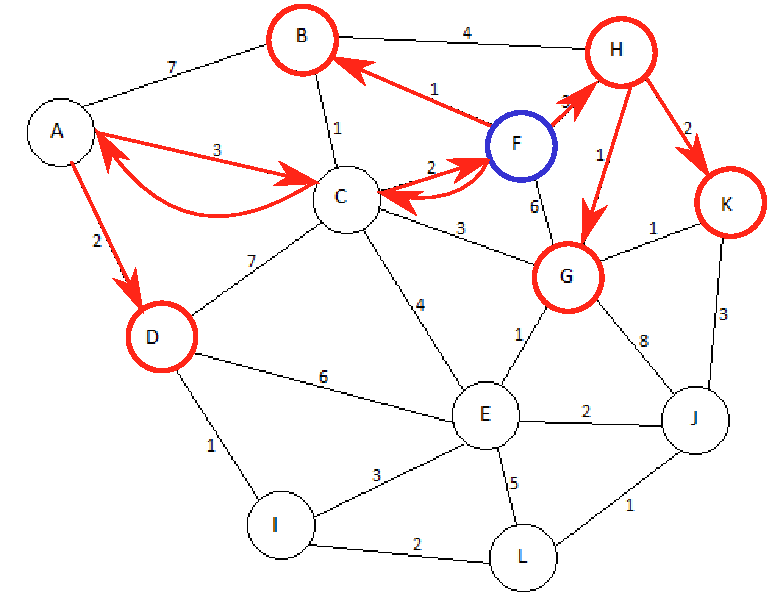
\includegraphics[width=\textwidth/2]{graph-a.pdf}
    \caption{Multicast Path starting in A}
  \end{figure}
	
	\subsection*{b) Multicast from C}
	
	\begin{figure}[h]
	  \centering
    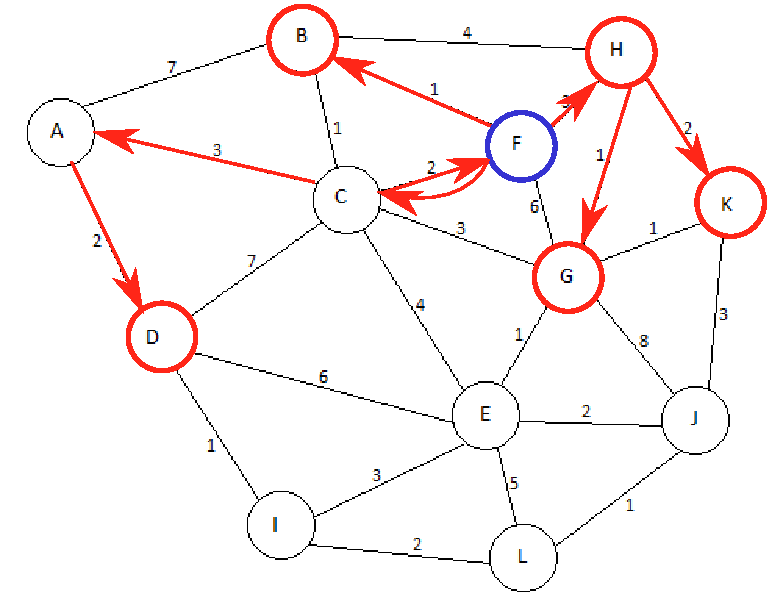
\includegraphics[width=\textwidth/2]{graph-b.pdf}
    \caption{Multicast Path starting in C}
  \end{figure}
	
	\end{document}
